\documentclass[dvipsnames,tikz]{standalone}
\usepackage{amsmath}
\usepackage{arevmath}
\usepackage{xcolor}
\usepackage{tikz}
\usetikzlibrary{calc}
\usetikzlibrary{decorations.pathreplacing,calligraphy,3d}
\usepackage{tikz-3dplot} 

\tikzset{main/.style={thick, circle, color=black}}

\begin{document}
	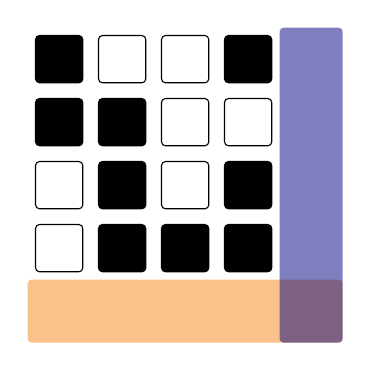
\begin{tikzpicture}[outer sep=0.05cm,node distance=0.8cm,]
		\tikzstyle{box} = [minimum size=0.6cm, 
		rounded corners=.05cm, 
		rectangle, 
		fill = white,
		draw = black]
		\tikzstyle{bbox} = [minimum size=0.6cm, 
		rounded corners=.05cm, 
		rectangle,
		fill = black,
		draw = black]
		\fill[BurntOrange, semitransparent, rounded corners=0.05cm] (-0.4,-3.6) rectangle (3.6,-2.8);
		\fill[NavyBlue, semitransparent, rounded corners=0.05cm] (2.8,-3.6) rectangle (3.6, 0.4);
		
		\node[bbox] (11) {};
		\node[box,right of=11] (12) {};
		\node[box,right of=12] (13) {};
		\node[bbox,right of=13] (14) {};
		%\node[box,right of=14] (15) {};
		
		\node[bbox,below of=11] (21) {};
		\node[bbox,right of=21] (22) {};
		\node[box,right of=22] (23) {};
		\node[box,right of=23] (24) {};
		%\node[box,right of=24] (25) {};
		
		\node[box,below of=21] (31) {};
		\node[bbox,right of=31] (32) {};
		\node[box,right of=32] (33) {};
		\node[bbox,right of=33] (34) {};
		%\node[box,right of=34] (35) {};
		
		\node[box,below of=31] (41) {};
		\node[bbox,right of=41] (42) {};
		\node[bbox,right of=42] (43) {};
		\node[bbox,right of=43] (44) {};
		%\node[bbox,right of=44] (45) {};
		
		%\node[box,below of=41] (51) {};
		%\node[bbox,right of=51] (52) {};
		%\node[bbox,right of=52] (53) {};
		%\node[bbox,right of=53] (54) {};
		%\node[bbox,right of=54] (55) {};
	\end{tikzpicture}
	
	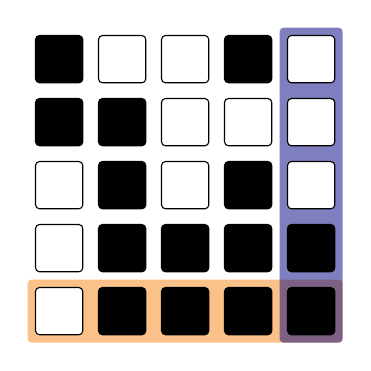
\begin{tikzpicture}[outer sep=0.05cm,node distance=0.8cm,]
		\tikzstyle{box} = [minimum size=0.6cm, 
						rounded corners=.05cm, 
						rectangle, 
						fill = white,
						draw = black]
		\tikzstyle{bbox} = [minimum size=0.6cm, 
						rounded corners=.05cm, 
						rectangle,
						fill = black,
						draw = black]
		\fill[BurntOrange, semitransparent, rounded corners=0.05cm] (-0.4,-3.6) rectangle (3.6,-2.8);
		\fill[NavyBlue, semitransparent, rounded corners=0.05cm] (2.8,-3.6) rectangle (3.6, 0.4);
		
		\node[bbox] (11) {};
		\node[box,right of=11] (12) {};
		\node[box,right of=12] (13) {};
		\node[bbox,right of=13] (14) {};
		\node[box,right of=14] (15) {};
		
		\node[bbox,below of=11] (21) {};
		\node[bbox,right of=21] (22) {};
		\node[box,right of=22] (23) {};
		\node[box,right of=23] (24) {};
		\node[box,right of=24] (25) {};
		
		\node[box,below of=21] (31) {};
		\node[bbox,right of=31] (32) {};
		\node[box,right of=32] (33) {};
		\node[bbox,right of=33] (34) {};
		\node[box,right of=34] (35) {};
		
		\node[box,below of=31] (41) {};
		\node[bbox,right of=41] (42) {};
		\node[bbox,right of=42] (43) {};
		\node[bbox,right of=43] (44) {};
		\node[bbox,right of=44] (45) {};
		
		\node[box,below of=41] (51) {};
		\node[bbox,right of=51] (52) {};
		\node[bbox,right of=52] (53) {};
		\node[bbox,right of=53] (54) {};
		\node[bbox,right of=54] (55) {};
	\end{tikzpicture}

	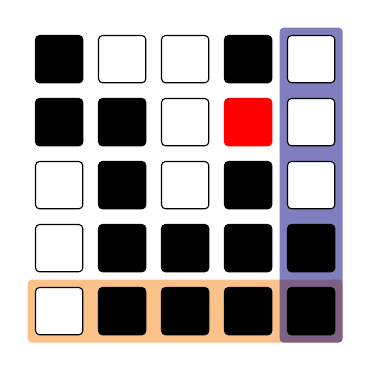
\begin{tikzpicture}[outer sep=0.05cm,node distance=0.8cm,]
		\tikzstyle{box} = [minimum size=0.6cm, 
		rounded corners=.05cm, 
		rectangle, 
		fill = white,
		draw = black]
		\tikzstyle{bbox} = [minimum size=0.6cm, 
		rounded corners=.05cm, 
		rectangle,
		fill = black,
		draw = black]
		\fill[BurntOrange, semitransparent, rounded corners=0.05cm] (-0.4,-3.6) rectangle (3.6,-2.8);
		\fill[NavyBlue, semitransparent, rounded corners=0.05cm] (2.8,-3.6) rectangle (3.6, 0.4);
		
		\node[bbox] (11) {};
		\node[box,right of=11] (12) {};
		\node[box,right of=12] (13) {};
		\node[bbox,right of=13] (14) {};
		\node[box,right of=14] (15) {};
		
		\node[bbox,below of=11] (21) {};
		\node[bbox,right of=21] (22) {};
		\node[box,right of=22] (23) {};
		\node[bbox,right of=23, draw=red, fill=red] (24) {};
		\node[box,right of=24] (25) {};
		
		\node[box,below of=21] (31) {};
		\node[bbox,right of=31] (32) {};
		\node[box,right of=32] (33) {};
		\node[bbox,right of=33] (34) {};
		\node[box,right of=34] (35) {};
		
		\node[box,below of=31] (41) {};
		\node[bbox,right of=41] (42) {};
		\node[bbox,right of=42] (43) {};
		\node[bbox,right of=43] (44) {};
		\node[bbox,right of=44] (45) {};
		
		\node[box,below of=41] (51) {};
		\node[bbox,right of=51] (52) {};
		\node[bbox,right of=52] (53) {};
		\node[bbox,right of=53] (54) {};
		\node[bbox,right of=54] (55) {};
	\end{tikzpicture}
\end{document}